\usetikzlibrary{positioning}

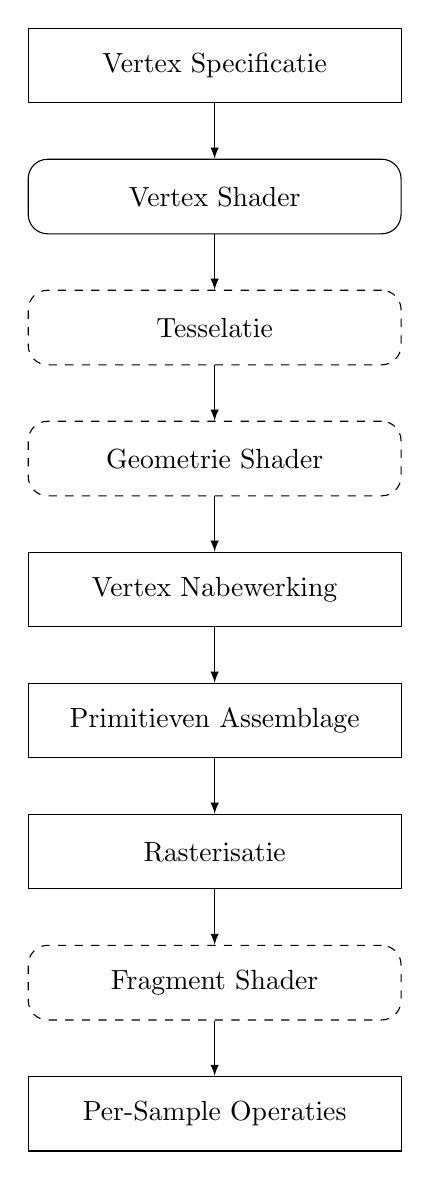
\begin{tikzpicture}[node distance=1cm, auto]
\tikzset{
    fixed/.style={rectangle, draw=black, text centered, minimum width={width("Primitieven Assemblage")+3em}, minimum height={height("Primitieven Assemblage")+2em}},
    prog/.style={rectangle, rounded corners=0.7em, draw=black, text centered, minimum width={width("Primitieven Assemblage")+3em}, minimum height={height("Primitieven Assemblage")+2em}},
    progOpt/.style={rectangle, rounded corners=0.7em, dashed, draw=black, text centered, minimum width={width("Primitieven Assemblage")+3em}, minimum height={height("Primitieven Assemblage")+2em}}
}  

% nodes
\node[fixed]                                        (vspec)      {Vertex Specificatie}; 
\node[prog, below=2em of vspec]     (vshader)  {Vertex Shader};
\node[progOpt, below=2em of vshader] (tes)          {Tesselatie};
\node[progOpt, below=2em of tes]         (gshader) {Geometrie Shader};
\node[fixed, below=2em of gshader] (vpp)        {Vertex Nabewerking};
\node[fixed, below=2em of vpp]        (pa)          {Primitieven Assemblage};
\node[fixed, below=2em of pa]          (rast)        {Rasterisatie};
\node[progOpt, below=2em of rast]        (fshader)  {Fragment Shader};
\node[fixed, below=2em of fshader] (pso)         {Per-Sample Operaties};

% arrows
\draw[-latex] (vspec) edge (vshader);
\draw[-latex] (vshader) edge (tes);
\draw[-latex] (tes) edge (gshader);
\draw[-latex] (gshader) edge (vpp);
\draw[-latex] (vpp) edge (pa);
\draw[-latex] (pa) edge (rast);
\draw[-latex] (rast) edge (fshader);
\draw[-latex] (fshader) edge (pso);

\end{tikzpicture}